\section{Project 6 - Geometric Transformation}

\subsection{Project Proposal}
Implement 4 geometric transform functions - rotate by a specified angle, translate by a given vector, scale by a given rate using nearest neighbor and scale by a given rate using bilinear interpolation.

\subsection{Preliminary}
\subsubsection{Spatial Transform}
A spatial transformation of an image is a geometric transformation of the image coordinate system. First we define the coordinate system in an image: \emph{axis-X} is from left to right while \emph{axis-Y} is from top to bottom. In a spatial transformation each point $(x,y)$ of origin image $A$ is mapped to point $(u,v)=(f_1(x,y), f_2(x,y))$ in a new coordinate system. \\
Affine transformation is any transformation that preserve collinearity and ratios of distances. Rotations, translations, magnifications, shears and their combinations are all affine transformations. Any single affine operation can be expressed as 
\begin{equation} \begin{bmatrix} u\\v\\1 \end{bmatrix} = 
\begin{bmatrix} c_{11} & c_{12} & c_{13} \\
c_{21} & c_{22} & c_{23} \\
0 & 0 & 1 \end{bmatrix} \begin{bmatrix}
x\\y\\1 \end{bmatrix} \end{equation}
We extend the 2D point to 3D in order to use a homogeneous matrix multiplication notation. Then we can represent translation, rotation, scaling under this notation. We denote the $3\times 3$ transformation matrix as $T$
\begin{equation} T= \begin{bmatrix} 1&0&x_0 \\ 0&1&y_0 \\ 0&0&1 \end{bmatrix} \text{Translation by }(x_0, y_0) \end{equation}
\begin{equation} T= \begin{bmatrix} s_1&0&0 \\ 0&s_2&0 \\ 0&0&1 \end{bmatrix} \text{Scale by $s_1$ and $s_2$} \end{equation}
\begin{equation} T= \begin{bmatrix} \cos \theta & -\sin \theta & 0 \\ \sin \theta & \cos \theta & 0 \\ 0&0&1 \end{bmatrix} \text{Rotate by $\theta$ (clockwise)} \end{equation}
\begin{equation} T= \begin{bmatrix} 1&\alpha&0 \\ 0&1&0 \\ 0&0&1 \end{bmatrix} \text{Horizontal shearing by }\alpha \end{equation}
\begin{equation} T= \begin{bmatrix} 1&0&0 \\ \beta&1&0 \\ 0&0&1 \end{bmatrix} \text{Vertical shearing by }\beta \end{equation}
Another advantage of matrix multiplication notation for affine transformation is that we can easily get composite affine transformation \begin{equation} T=\prod_i T_i \end{equation} as well as the inverse transformation $T^{-1}$
\subsubsection{Interpolation}
After conduct geometric spatial transformation, the new grid points may not locate exactly on grid points in the new coordinate system. Interpolation is needed in this kind situation to find out th value of the grid points in the new coordinate system. Here, we talk about two methods of interpolation - nearest neighbor interpolation and bilinear interpolation.\\ 
Nearest neighbor interpolation is the simplest and fastest interpolation method. In practice, we just use the $(x,y,1)^T = round(T^{-1}(u,v,1)^T)$ as nearest neighbor interpolation.\\
In bilinear interpolation, we first calculate $(x',y')$ in $O_{xy}$ which is the original phase of a grid point $(u,v)$ in $O_{uv}$. Then find out the smallest rectangle that surround $(x', y')$ which is formed by 4 grid points $\{(x_0,y_0), (x_1,y_1), (x_2,y_2), (x_3,y_3)\}$ in $O_xy$. Thus we calculate the value at grid point $(x', y')$ as well as $(u,v)$ in $O_{uv}$ in the following way including 2 level of linear interpolation: \begin{equation} g_{0,1}(x',y')=\frac{x_1-x'}{x_1-x_0}f(x_0, y_0) + \frac{x'-x_0}{x_1-x_0}f(x_1, y_1)\end{equation} \begin{equation} g_{3,2}(x',y')=\frac{x_2-x'}{x_2-x_3}f(x_3, y_3) + \frac{x'-x_3}{x_2-x_3}f(x_2, y_2)  \end{equation} \begin{equation} g(x',y')=\frac{y_2-y'}{y_2-y_1}g_{0,1}(x',y') + \frac{y'-y_1}{y_2-y_1}g_{3,2}(x',y')  \end{equation}

\subsection{Experiment}
In this experiment we use Fig.\ref{fig:origin} for testing.
\begin{figure}[h]
	\centering
	\begin{subfigure}[b]{0.45\linewidth}
		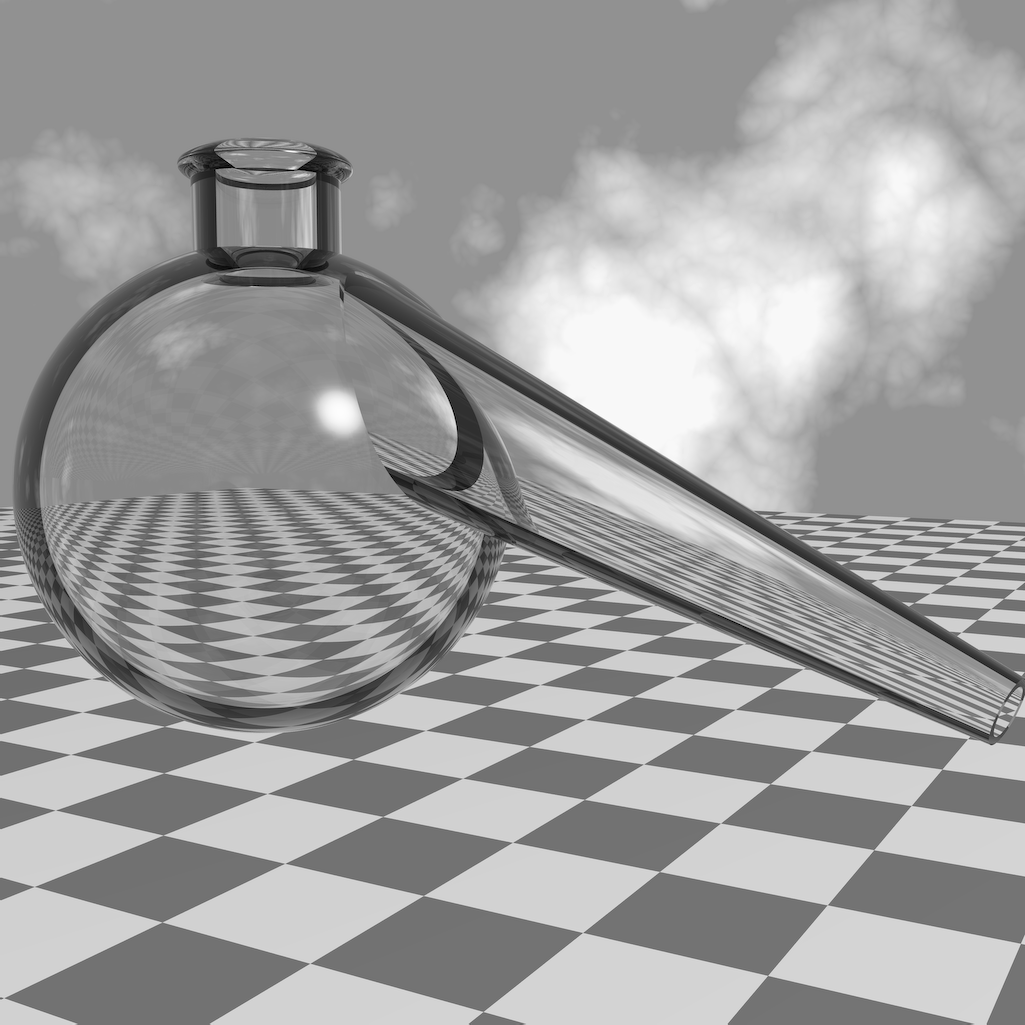
\includegraphics[width=\linewidth]{myfigure/p6/ray_trace_bottle.png}
		\caption{}
		\label{fig:origin1}
	\end{subfigure}
	\caption{Origin test image}
  	\label{fig:origin}
\end{figure}

\textbf{Translate} The image is translated by 100 pixel at right and by 200 pixel down. The result is display in Fig.\ref{fig:translate}. 
\begin{figure}[h!]
	\centering
	\begin{subfigure}[b]{0.45\linewidth}
		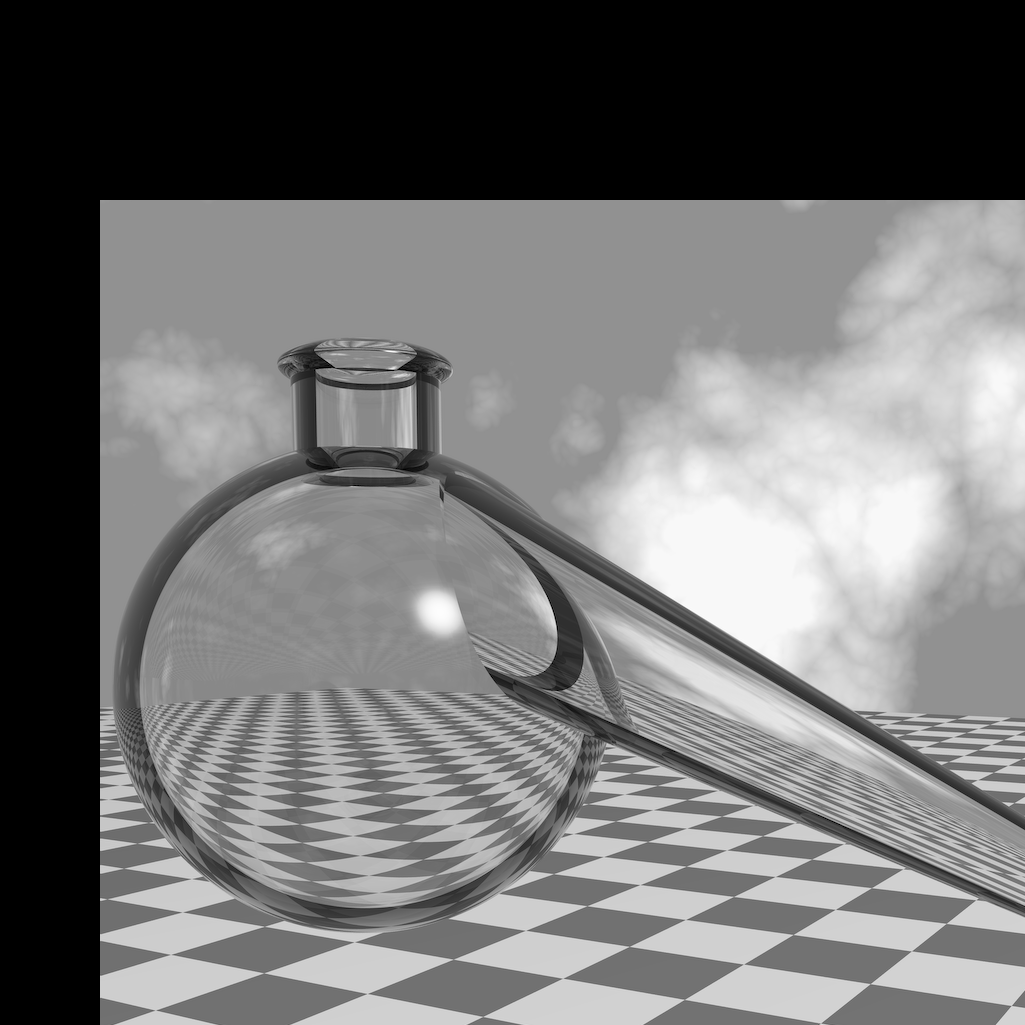
\includegraphics[width=\linewidth]{myfigure/p6/translation_ne.png}
		\caption{Use nearest neighbor interpolation.}
		\label{fig:translate_ne}
	\end{subfigure}
  	\begin{subfigure}[b]{0.45\linewidth}
		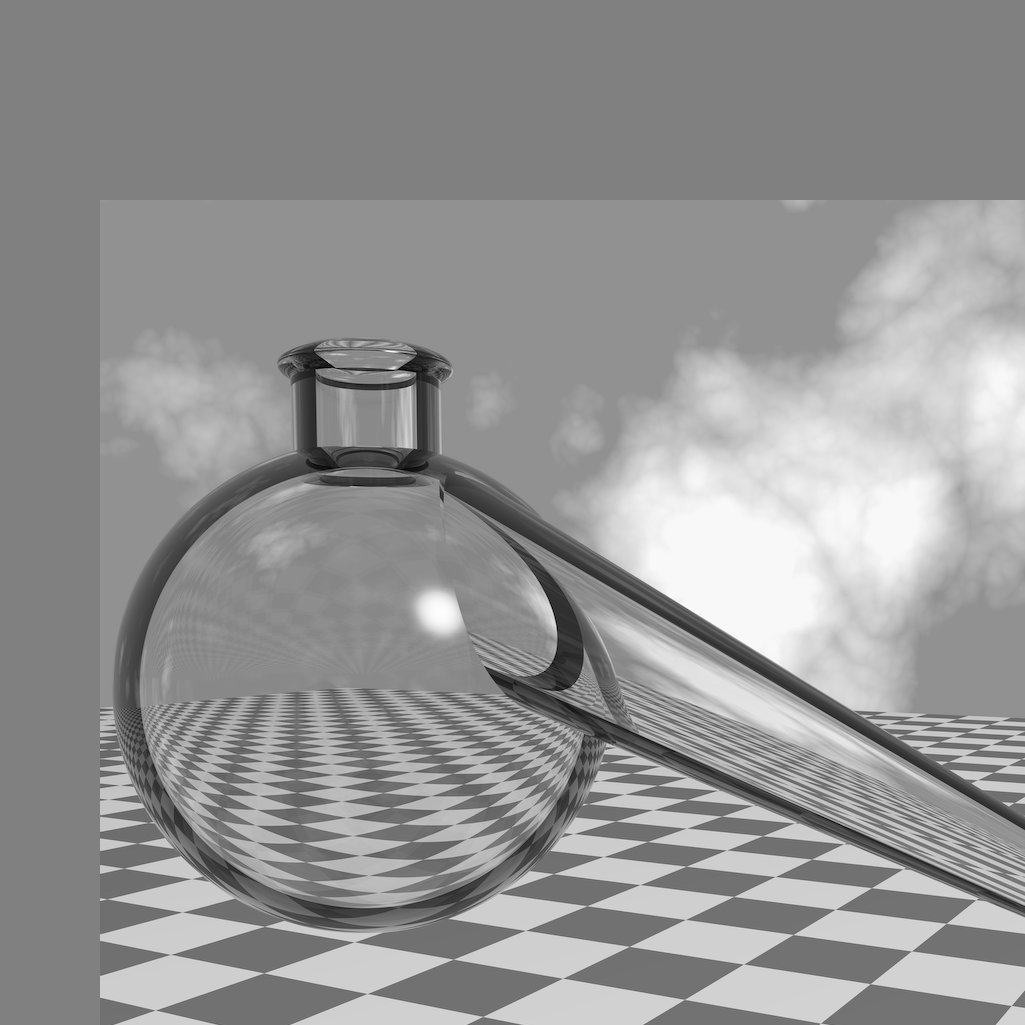
\includegraphics[width=\linewidth]{myfigure/p6/translation_bi.png}
		\caption{Use bilinear interpolation.}
		\label{fig:translate_bi}
	\end{subfigure}
  	\caption{Results of translate 100 from left to right and 200 down.}
  	\label{fig:translate}
\end{figure}

\textbf{Rotation} The image is rotated by $\pi /6$ clockwise. The result is display in Fig.\ref{fig:rotate}. 
\begin{figure}[h!]
	\centering
	\begin{subfigure}[b]{0.45\linewidth}
		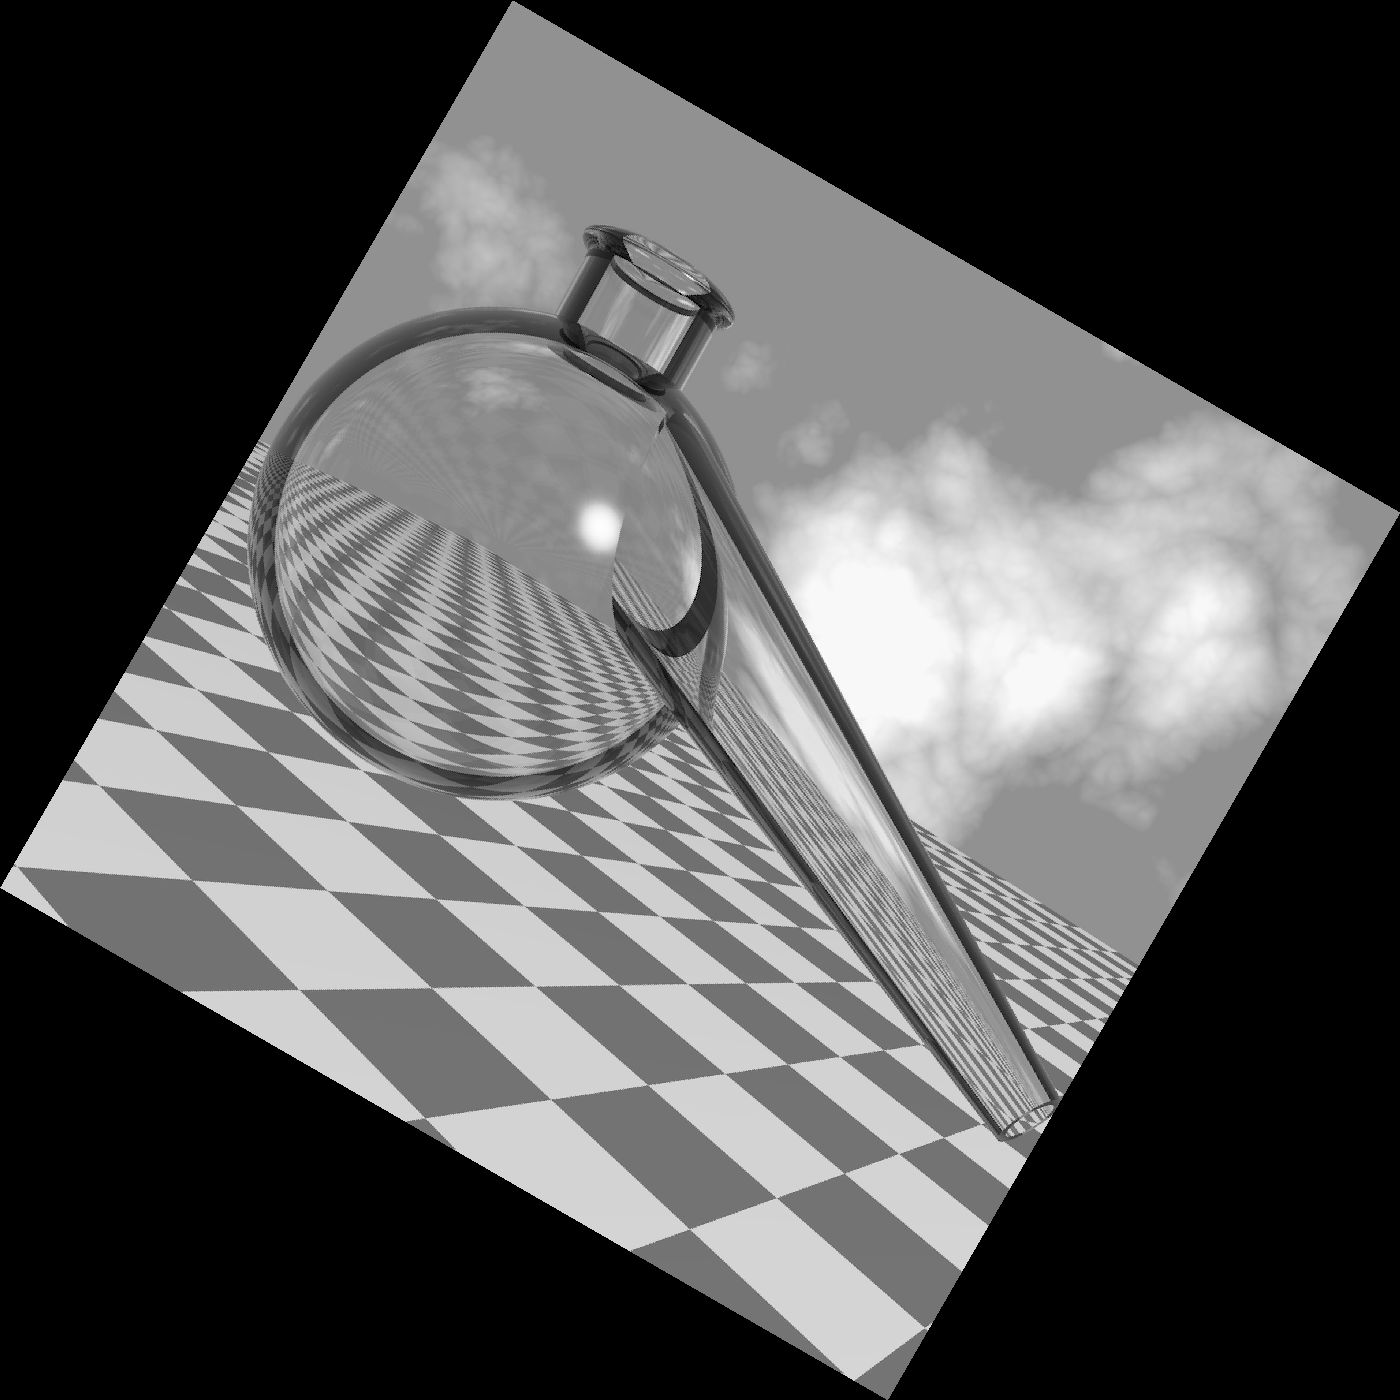
\includegraphics[width=\linewidth]{myfigure/p6/rotation_ne.png}
		\caption{Use nearest neighbor interpolation.}
		\label{fig:rotate_ne}
	\end{subfigure}
  	\begin{subfigure}[b]{0.45\linewidth}
		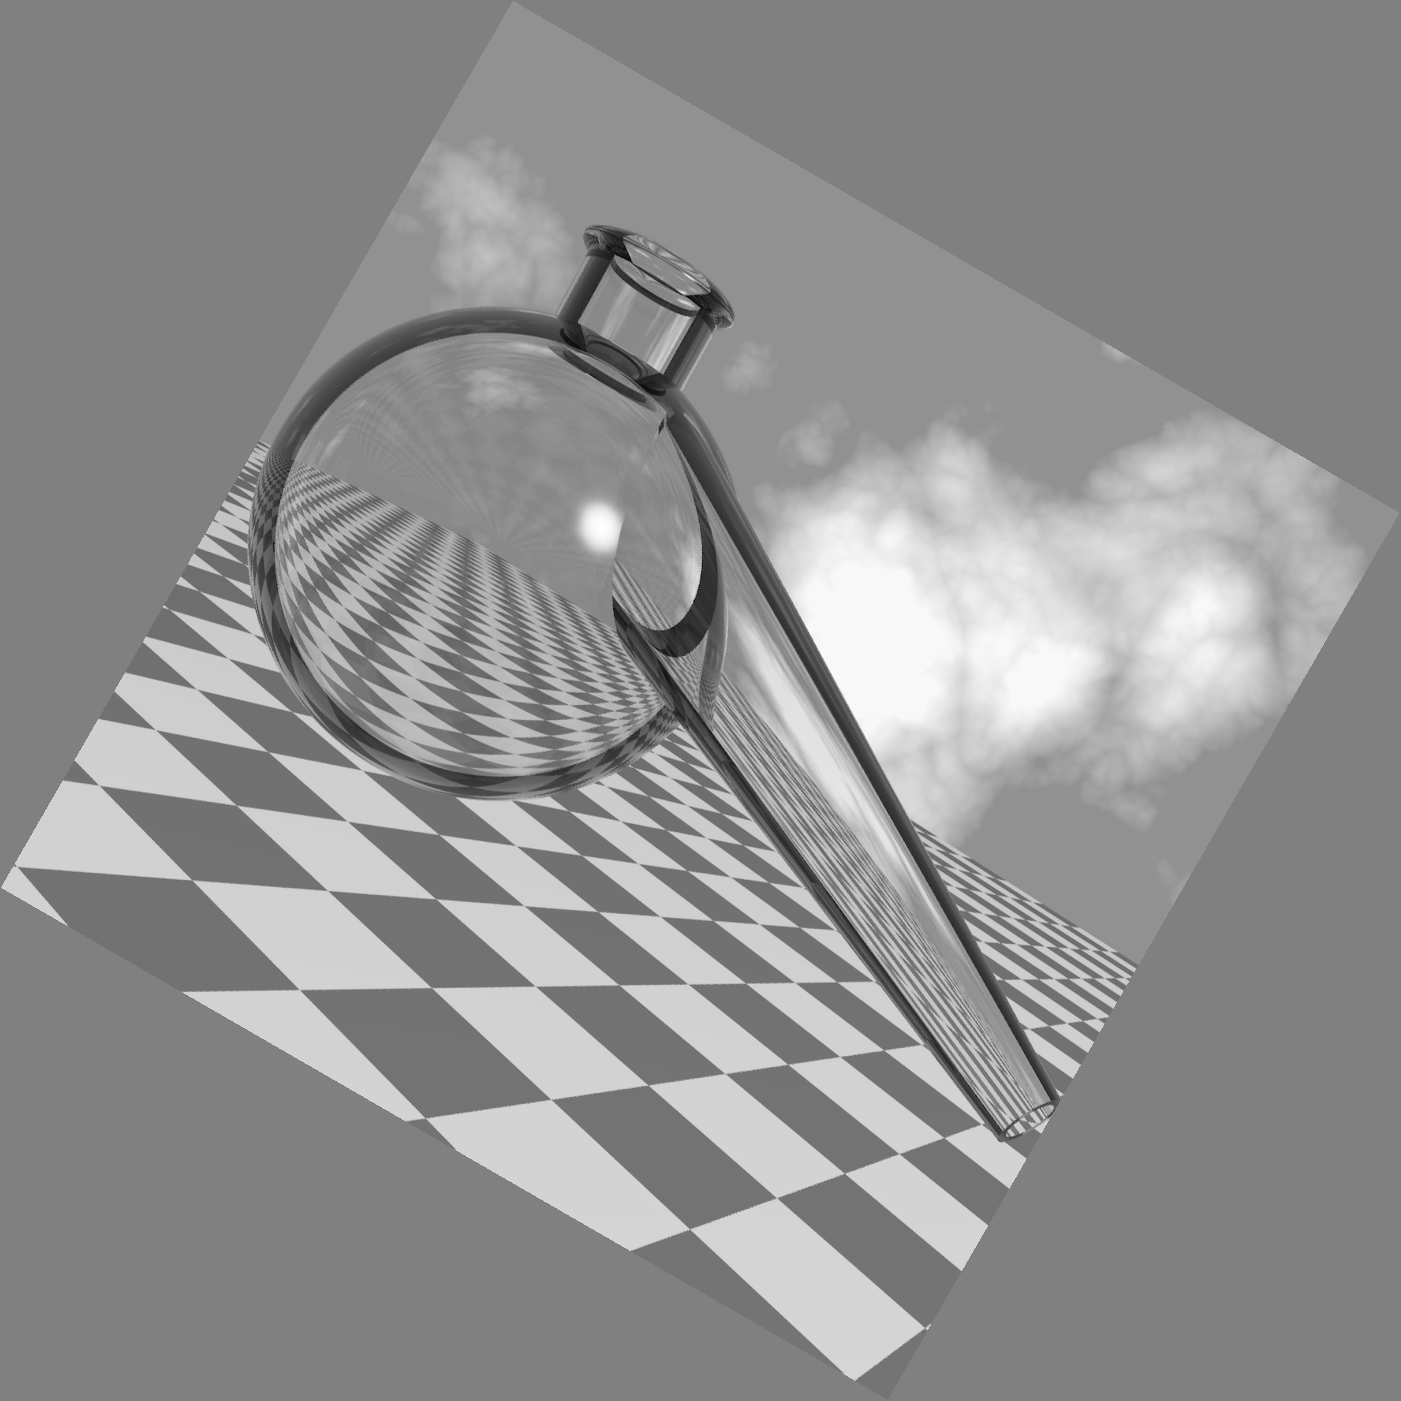
\includegraphics[width=\linewidth]{myfigure/p6/rotation_bi.png}
		\caption{Use bilinear interpolation.}
		\label{fig:rotate_b}
	\end{subfigure}
  	\caption{Results of rotation. $\pi/6$ clockwise.}
  	\label{fig:rotate}
\end{figure}


\textbf{Scaling} The image is scaled by 1.5 at axis-x and by 2 at axis-y. The result is display in Fig.\ref{fig:rotate}.
\begin{figure}[h!]
	\centering
	\begin{subfigure}[b]{0.45\linewidth}
		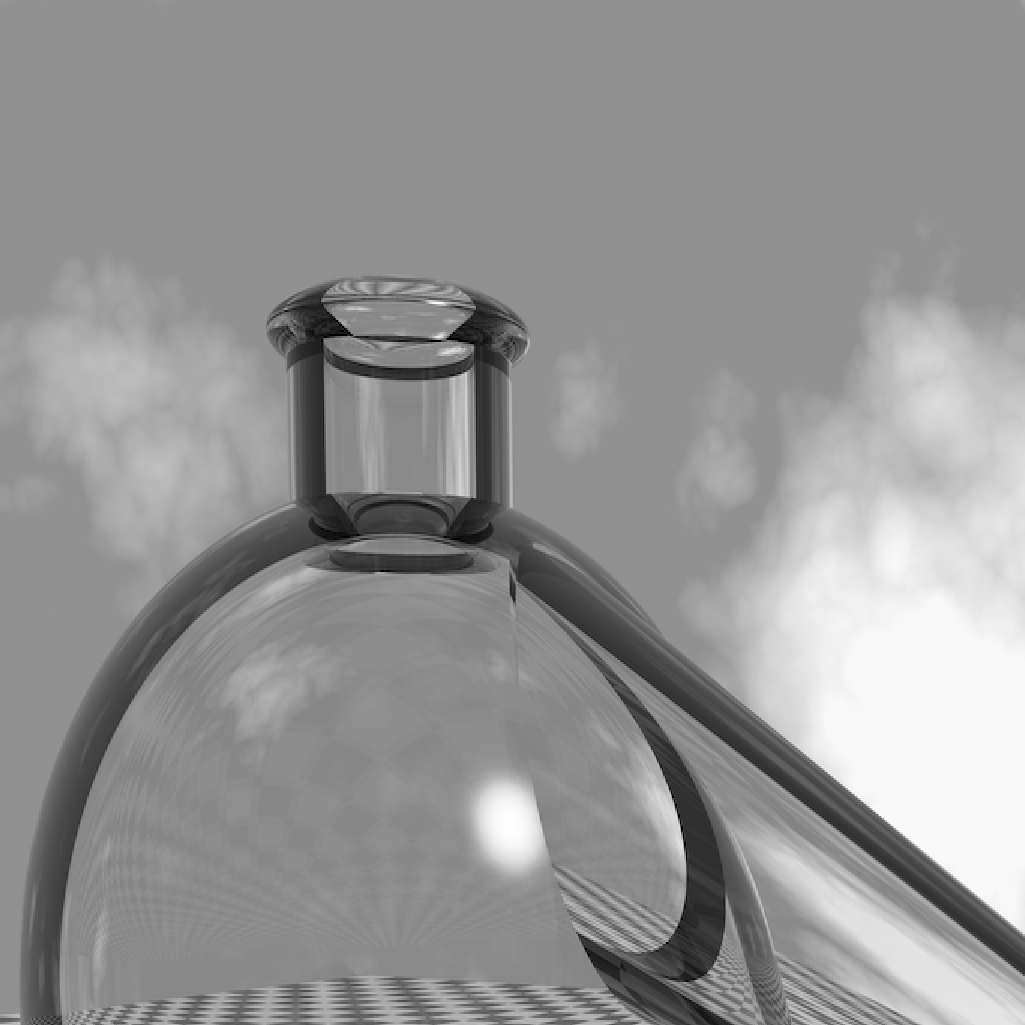
\includegraphics[width=\linewidth]{myfigure/p6/scale_ne.png}
		\caption{Use nearest neighbor interpolation.}
		\label{fig:scale_ne}
	\end{subfigure}
  	\begin{subfigure}[b]{0.45\linewidth}
		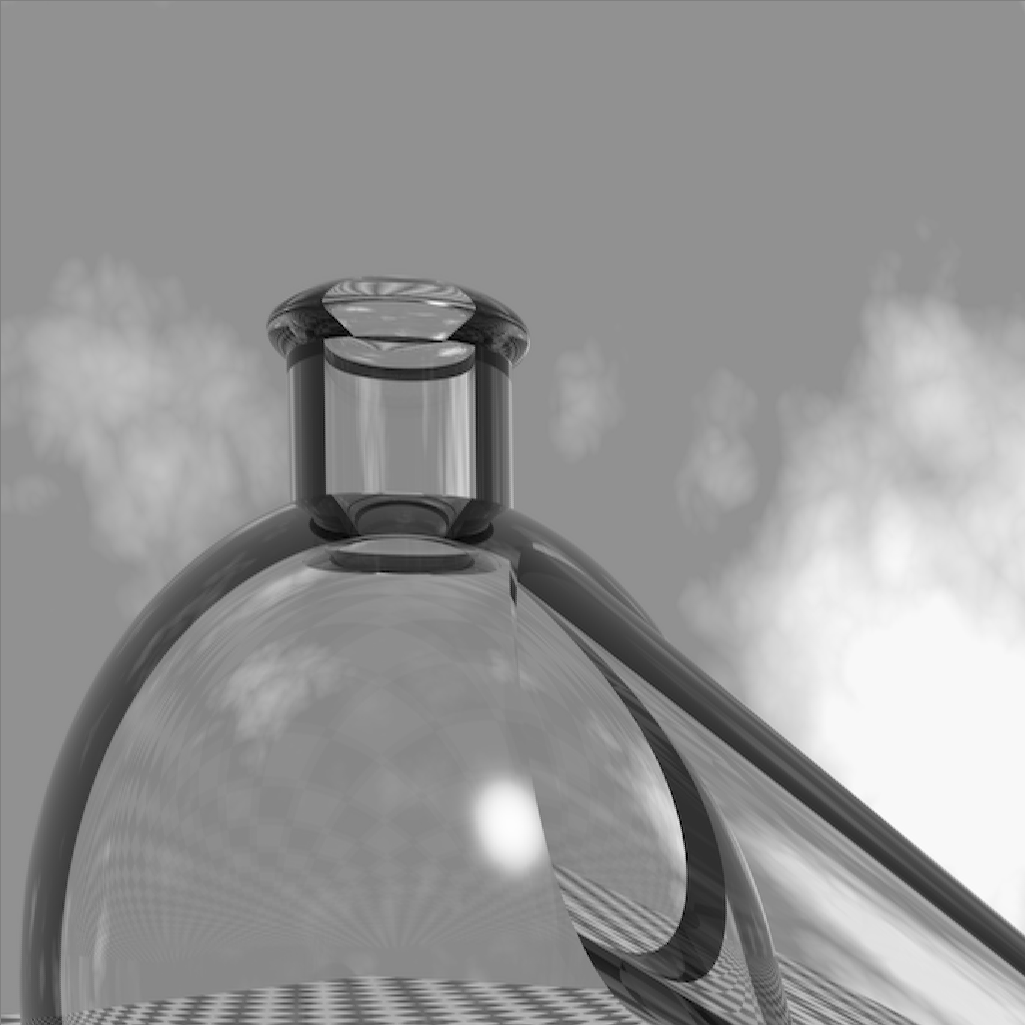
\includegraphics[width=\linewidth]{myfigure/p6/scale_bi.png}
		\caption{Use bilinear interpolation.}
		\label{fig:scale_bi}
	\end{subfigure}
  	\caption{Results of scaling. Times 1.5 at axis-X and times 2 at axis-Y.}
  	\label{fig:scale}
\end{figure}

\subsection{Implementation}
The main part of this implementation is on the function \emph{mytransform}. The input parameters are three necessary parameters - input image, $3\times 3$ affine transform matrix, interpolation method and 3 optional parameters - horizontal and vertical display boundaries and filling colors for empty pixels. \\

The idea is simple: First, find out the output image's size based only on the transform matrix and input image. The approach is to calculate the coordinates for four rectangle vertices. After consider the user defined boundary, we get the size of final output rectangle range. Then use the each grid coordinate $(u,v)$ to calculate the corresponding $(x,y)$ in input. After get $(x,y)$, get the pixel value $g(u,v)$ according to the interpolation methods. To get the little square where $(x,y)$ is in, another function \emph{bilinear\_rect} is written.\\

The code of \emph{mytransform} and \emph{bilinear\_rect}is listed below:
\lstset{language=Matlab}
\begin{lstlisting}
function [ imgg ] = mytransform( imgf, matT, interpolation, varargin )
%MYTRANSFORM 
%  
ip = inputParser;
ip.addParameter('fillValue', 0);
ip.addParameter('boundX', [0, 0]);
ip.addParameter('boundY', [0, 0]);
ip.parse(varargin{:});
para=ip.Results;
    
boundX = para.boundX;
boundY = para.boundY;
fillValue = para.fillValue;
setBound = 1;
if (boundX(2)==boundX(1) || boundY(1)==boundY(2))
    setBound=0;
end

[M, N] = size(imgf);
X = [1 N N 1];
Y = [1 1 M M];
tmp = matT * [X; Y; ones(1,4)];

minX = floor(min(tmp(1,:)));
minY = floor(min(tmp(2,:)));
maxX = ceil(max(tmp(1,:)));
maxY = ceil(max(tmp(2,:)));

if(setBound==1)
    minX = boundX(1);
    maxX = boundX(2);
    minY = boundY(1);
    maxY = boundY(2);
end
imgg = zeros(maxY-minY, maxX-minX);

for i=(minY:maxY)
    for j=(minX:maxX)
        tmp = matT \ [j;i;1];
        u = tmp(1);
        v = tmp(2);    
        if(isequal('bilinear', interpolation))
            [X, Y, out] = bilinear_rect(tmp, M, N);
            if(out==1)
            	imgg(i-minY+1, j-minX+1) = fillValue;
            	continue;
            end
            g_12 = (X(2)-u)/(X(2)-X(1))*imgf(Y(1),X(1)) + (u-X(1))/(X(2)-X(1))*imgf(Y(1),X(1));
            g_34 = (X(3)-u)/(X(3)-X(4))*imgf(Y(4),X(4)) + (u-X(4))/(X(3)-X(4))*imgf(Y(3),X(3));
            imgg(i-minY+1, j-minX+1) = (Y(3)-v)/(Y(3)-Y(2))*g_12 + (v-Y(2))/(Y(3)-Y(2))*g_34;
        end
        if(isequal('nearest', interpolation))
        	if(round(u)>=1 && round(u)<=N && round(v)>=1 && round(v)<=M)
            	imgg(i-minY+1, j-minX+1) = imgf(round(v), round(u));
            end
        end
    end
end
end

function [ X, Y, out ] = bilinear_rect(orig_p, M, N)
u = orig_p(1);
v = orig_p(2);
X = zeros(1,4);
Y = zeros(1,4);
X(1) = floor(u);
X(3) = ceil(u);
if(X(1)==X(3))
	X(3) = X(1)+1;
end
Y(1) = floor(v);
Y(3) = ceil(v);
if(Y(1)==Y(3))
	Y(3) = Y(1)+1;
end
out = 0;
if(X(1)<1 || X(3)>N || Y(1)<1 || Y(3)>M)
	out = 1;
end
X(4) = X(1);
X(2) = X(3);
Y(4) = Y(3);
Y(2) = Y(1);
end
\end{lstlisting}

\subsection{Discussion}
When we are implementing the coordinate transform, we should pay attention to that the coordinate of an image is not the same as the one in mathematics. For example, for efficiency reason, we usually loop 'y' outer and loop 'x' inner. Hence, be careful to use the loop variables correctly while indexing the image matrix. Another difference is that in mathematics, we use counter-clock direction as positive direction for rotation while here we use clockwise direction as positive direction.
In this experiment, I didn't see large difference between bilinear interpolation and nearest neighbor interpolation. However, in practice, we should consider the efficiency and effects when we are choosing the proper interpolation algorithm.
























